\section{Benchmark design}
\label{sec:benchmark}

With a cleaned dataset (§\ref{sec:data_curation}) and a calibrated
noise floor (§\ref{sec:aleatoric}), we can now build the benchmark
itself.  \scthree{} is designed to answer three distinct generalisation
questions simultaneously: can a model predict (i) a new
$(\mathrm{solute}, \mathrm{solvent})$ pair in a familiar solvent,
(ii) the same solute in a solvent it has never seen, and
(iii) a new solute against consensus-calibrated labels with per-point
uncertainty $\sigma$?  Each question corresponds to a separate
evaluation set.  The construction is: a \emph{tier-test pool} with
consensus labels from multi-source agreement, and a \emph{training
pool} drawn from the complement that is further split by
solvent-frequency into in-distribution (Train, Eval) and
out-of-distribution (OOD) sets.

\subsection{Tier construction}
\label{sec:tiers}

The tiers are the benchmark's evaluation with calibrated ground truth
and $\sigma$.  They are built from the \numval{481} multi-source pairs
that survive
(i) the copycat merging of §\ref{sec:source}, (ii) the Hall-of-Shame
exclusion, and (iii) the fit-quality gate of §\ref{sec:apelblat}.  For
each eligible pair we compute the pair MAE (equation~\ref{eq:mae_pair})
and assign it to every tier whose MAE threshold it satisfies:

\begin{center}
\renewcommand{\arraystretch}{1.08}\small
\begin{tabular}{@{}lll@{}}
\toprule
Tier   & Pair MAE threshold          & Meaning \\
\midrule
\textbf{Gold}   & $\leq 0.1$ log S    & consensus labels disagree by at most $\sim\epsA$ \\
\textbf{Silver} & $\leq 0.2$ log S    & within a factor of $\sim 2\epsA$ \\
\textbf{Bronze} & $\leq 0.5$ log S    & within a factor of $\sim 5\epsA$ \\
\bottomrule
\end{tabular}
\end{center}

The tiers are \emph{nested}: $\text{Gold} \subset \text{Silver} \subset
\text{Bronze}$.  The naming is designed so that a \textbf{tighter tier
label corresponds to a better-characterised ground truth}, not to a
harder modelling task.  A model evaluated on Gold is being compared
against the tightest available reference labels; Bronze is a broader
net that keeps more pairs at the cost of looser consensus.

\paragraph{Consensus labels.}
For each $(\mathrm{solute}, \mathrm{solvent}, T)$ triple in a tier pair,
we evaluate every contributing independence group's Apelblat /
van't-Hoff fit at $T$ and define the consensus label as the mean of
those evaluations, excluding Hall-of-Shame groups.  The per-point
uncertainty $\sigma$ is the standard deviation across the same set of
evaluations.  When fewer than two groups contribute at a given $T$,
$\sigma$ is undefined and the row carries a hard label with no
uncertainty; this happens on \numval{14.4}\,\% of tier rows overall.

\paragraph{Uncertainty floor.}
A standard deviation from two nearly-identical fits can underestimate
true measurement spread.  We therefore floor $\sigma$ at $0.012$ log S
($\approx \epsA / 10$) --- the median Apelblat fit RMSE
(§\ref{sec:apelblat}) --- to prevent a handful of suspiciously-tight
$\sigma$s from dominating $Z$-normalised losses.

\paragraph{Tier statistics.}
Table~\ref{tab:tiers} shows size and $\sigma$ distribution per tier.
Median $\sigma$ ranges from \numval{0.019} (Gold) through \numval{0.024}
(Silver) to \numval{0.031} (Bronze); the Gold tail is much shorter
($P_{95} = \numval{0.078}$ vs Bronze $P_{95} = \numval{0.245}$),
reflecting the tighter pair-MAE cap.  Figure~\ref{fig:tier_sigma} shows
the full $\sigma$ distribution per tier: the Gold distribution is
entirely below Bronze's tail.

\begin{table}[h]
\centering\small
\caption{SC$^{3}$ tier composition and $\sigma$ statistics.  Nested:
Gold $\subset$ Silver $\subset$ Bronze.  $\sigma$-coverage is the
fraction of tier rows with a defined per-point uncertainty; remaining
rows have a hard label only.}
\label{tab:tiers}
\begin{tabular}{@{}lrrrr cccc@{}}
\toprule
Tier   & rows  & pairs & solutes & solvents
       & $\sigma$-cov. & median $\sigma$ & mean $\sigma$ & $P_{95}\ \sigma$ \\
\midrule
Gold   & 4\,507 & 335 & 129 & 26 & 76.5\%  & 0.019 & 0.028 & 0.078 \\
Silver & 5\,475 & 400 & 141 & 27 & 76.9\%  & 0.024 & 0.042 & 0.130 \\
Bronze & 6\,331 & 469 & 148 & 30 & 77.1\%  & 0.031 & 0.066 & 0.245 \\
\bottomrule
\end{tabular}
\end{table}

\begin{figure}[t]
\centering
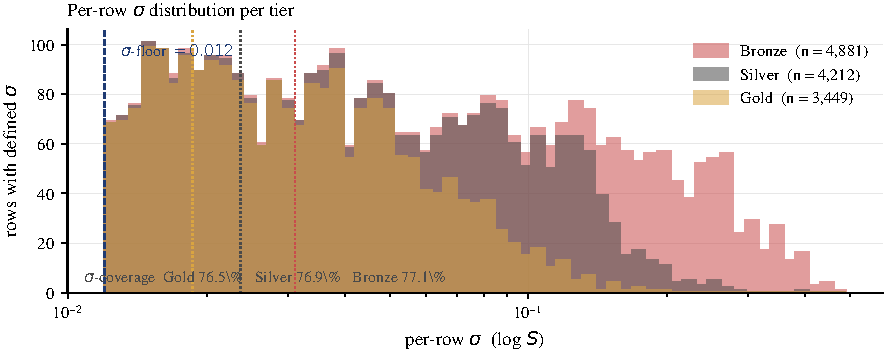
\includegraphics[width=0.9\linewidth]{figures/fig_tier_sigma.pdf}
\caption{Per-row $\sigma$ distribution in the three nested tiers, log-$\sigma$
 axis.  Dashed vertical line at the $\sigma$-floor $= 0.012$ log S; dotted
 lines mark per-tier medians.  Gold's distribution is concentrated between
 the floor and $\sim 0.03$ log S; Bronze has a much longer tail out to
 $\sigma > 0.2$ log S.  $\sigma$-coverage is near-identical across tiers
 ($\sim 77\,\%$), so the tail difference is about \emph{quality} of
 uncertainty, not quantity.}
\label{fig:tier_sigma}
\end{figure}

\subsection{Training, evaluation, and OOD splits}
\label{sec:splits}

Tiers consume only a thin slice of the cleaned pool; the complement
forms the training and in-distribution test sets, and the long-tail
solvents become the out-of-distribution test set.  The
\numval{148} solutes that appear in any tier are fully excluded from
the training pool at the $(\mathrm{solute}, \mathrm{solvent}, T)$
level --- no row containing such a solute survives into Train, Eval,
or OOD.
The remaining \numval{80\,312} rows are split by solvent frequency:

\begin{itemize}[leftmargin=1.25em,itemsep=1pt]
\item \textbf{Top-25 solvents} (ranked by training-pool row count,
covering \numval{85.1\,\%} of the training pool) form the
\emph{in-distribution} region.  Within this region, \numval{10\,\%} of
each solvent's solute list is held out as \textbf{Eval}; the remainder
is \textbf{Train}.
\item \textbf{Remaining \numval{181} solvents} form the \textbf{OOD}
set.  By construction a model will never have been trained on any of
these solvents, which tests whether it can generalise across the
solvent axis.
\end{itemize}

Table~\ref{tab:splits} summarises the final composition.

\begin{table}[t]
\centering\small
\caption{SC$^{3}$ splits and tiers.  All six evaluation subsets have
zero solute overlap with training (see Table~\ref{tab:antileakage}).
Solvent overlap with Train is intentional for Eval (in-distribution)
and tiers (calibrated labels); OOD has zero solvent overlap with Train
by construction.}
\label{tab:splits}
\begin{tabular}{@{}llrrrr@{}}
\toprule
& Role                           & rows     & solutes & solvents & (solute, solvent) pairs \\
\midrule
\multicolumn{6}{l}{\textit{Training pool (\numval{80\,312} rows after tier exclusion)}} \\
Train  & training set                   & 61\,403  & 1\,144  & 25       & 6\,840 \\
Eval   & new-pair, in-distribution      &  6\,969  &    534  & 25       &    771 \\
OOD    & new-solvent (151 unseen)       & 11\,940  &    586  & 161      &  1\,450 \\
\midrule
\multicolumn{6}{l}{\textit{Tier test pool (solutes fully absent from training pool)}} \\
Gold   & tight consensus, $\sigma$-cal.  &  4\,507  &    129  &  26      &    335 \\
Silver & looser consensus, $\sigma$-cal. &  5\,475  &    141  &  27      &    400 \\
Bronze & broadest, $\sigma$-cal.         &  6\,331  &    148  &  30      &    469 \\
\bottomrule
\end{tabular}
\end{table}

\paragraph{Generalisation axes exposed.}
The three evaluation sets test distinct notions of generalisation:

\begin{itemize}[leftmargin=1.25em,itemsep=1pt]
  \item \textbf{Eval} tests \emph{new (solute, solvent) pairs} in
    already-seen solvents.  A model must interpolate across the
    solute axis.
  \item \textbf{OOD} tests \emph{new solvents} (the \numval{161}
    long-tail solvents).  Solute may have been seen in a different
    solvent, but the target solvent is unseen.  Some solvents have few
    measurements; we therefore report OOD metrics with the per-solvent
    split-out explicitly (§\ref{sec:metrics}).
  \item \textbf{Gold / Silver / Bronze} test \emph{new solutes} against
    calibrated consensus labels with $\sigma$.  Any of the 148 tier
    solutes has been removed from Train/Eval/OOD, so all tier tests
    are solute-level out-of-distribution.
\end{itemize}

\paragraph{Anti-leakage verification.}
Every overlap that must be zero, is zero (Table~\ref{tab:antileakage}).
Solute overlap between Train and Eval is expected to be positive
($\numval{520}$ solutes) because Eval is a held-out slice of the
in-distribution solute--solvent grid; pair-level overlap between Train
and Eval remains zero by construction of the hold-out.

\begin{table}[h]
\centering\small
\caption{Anti-leakage verification.  Every cell reports the count of
(solute, solvent) pair overlaps between two splits.  Zero everywhere
except the two off-diagonal entries that are expected to share solutes
but never pairs (shaded).  All checks pass.}
\label{tab:antileakage}
\begin{tabular}{@{}lcccccc@{}}
\toprule
          & Train & Eval & OOD & Gold & Silver & Bronze \\
\midrule
Train     & ---   & 0    & 0   & 0    & 0      & 0      \\
Eval      & 0     & ---  & 0   & 0    & 0      & 0      \\
OOD       & 0     & 0    & --- & 0    & 0      & 0      \\
Gold      & 0     & 0    & 0   & ---  & nested & nested \\
Silver    & 0     & 0    & 0   & nested & ---  & nested \\
Bronze    & 0     & 0    & 0   & nested & nested & ---   \\
\bottomrule
\end{tabular}
\end{table}

\begin{figure}[h]
\centering
\figplaceholder{fig_splits_diagram.pdf}{0.30}{%
  Two-axis schematic of the leakage-hard splits.  Horizontal axis = solvent
  set (25 ID solvents on the left, 161 OOD solvents on the right);
  vertical axis = solute set (training-pool solutes vs.\ tier solutes,
  fully disjoint).  Train (top-left), Eval (top-left held-out pairs),
  OOD (top-right, ID solutes in unseen solvents), and tiers
  (bottom-left, tier solutes in ID solvents with calibrated
  $\sigma$).  Cell row counts: Train $61\,403$, Eval $6969$,
  OOD $11\,940$, Bronze $6331$.  Use coloured rectangles with row counts
  inside and a legend identifying each split.%
}
\caption{Three generalisation axes the splits expose.  \emph{Eval}
tests new (solute, solvent) pairs in familiar solvents;
\emph{OOD} tests unseen solvents; the tiers test new solutes in
familiar solvents \emph{with calibrated $\sigma$}.}
\label{fig:splits_diagram}
\end{figure}
